\documentclass[aspectratio=169, usenames, dvipsnames]{beamer}

\usepackage{xcolor}
\usepackage[normalem]{ulem} % for strikethrough text

% set up minted
\usepackage{minted}
\setminted{autogobble=true, linenos=false, fontsize=\footnotesize}
\usemintedstyle{friendly}

\definecolor{rustcolor}{rgb}{0.95,0.95,0.95}

% LAST import: menukeys
% \usepackage{menukeys}
% \renewmenumacro{\menu}[>]{roundedmenus}

% for semi transparent text
\newcommand{\semitransp}[2][35]{\textcolor{fg!#1}{#2}}

% setup for footnotes...
\addtobeamertemplate{footnote}{\vspace{-8pt}\advance\hsize-0.5cm}{\vspace{8pt}}
\makeatletter
\renewcommand*{\footnoterule}{\kern -3pt \hrule \@width 2in \kern 10.6pt}
\setbeamerfont{footnote}{size=\tiny}

\title{Ohua as STM Alternative for Shared State Applications}
\subtitle{Master Defense}
\date{25th August 2020}
\author{Felix Wittwer}

\usetheme{ccc}

\begin{document}

\begin{frame}
\titlepage
\end{frame}

%\begin{frame}{Ohua\footnotemark[1]}
  %\begin{columns}
    %\begin{column}{0.7\textwidth}
      %Framework for implicit parallel programming:\\[.55\baselineskip]
      %\begin{itemize}
        %\item<2-> Derives dataflow graph from algorithm file
        %\item<3-> Runs optimizations on graph to exploit parallelism at compile time
        %\item<4-> Generates native runtime code
      %\end{itemize}
      %% TODO: Zusätzlichen Punkt, der Ohua besser verkauft für dieses Problem.
    %\end{column}
    %\begin{column}{0.25\textwidth}
      %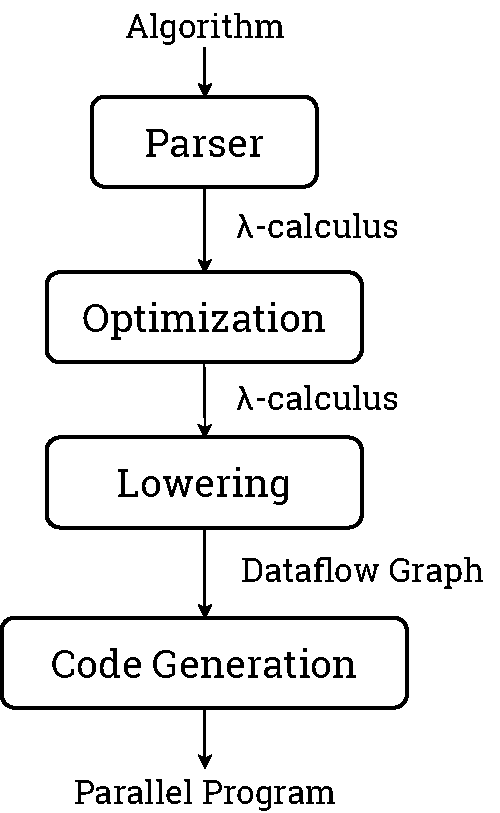
\includegraphics[width=\textwidth,height=\textheight,keepaspectratio]{img/ohua}
    %\end{column}
  %\end{columns}
  %% TODO: Chart showing what it does (?), bullet point that we want to make a comparison
  %% \vfill

  %% \uncover<4->{\textbf{Challenges:}}
  %% \begin{itemize}
  %% \item<4->{Ohua does not provide primitives for transactions}
  %%   \begin{itemize}
  %%   \item<5-> Use \texttt{smap} and shared state
  %%   \end{itemize}
  %% \item<6-> Problem: Collision handling
  %%   \begin{itemize}
  %%   \item<7-> Collect failed jobs and call transaction recursively
  %%   \end{itemize}
  %% \end{itemize}
  %\footnotetext[1]{Ertel et al. "Towards Implicit Parallel Programming for Systems." dissertation, 2019.}
%\end{frame}

%\begin{frame}{Throwback: Labyrinth Benchmark}
  %\begin{columns}
    %\begin{column}{0.5\textwidth}
      %\textbf{Given:} 3D maze, pairs of points\\[\baselineskip]

      %\uncover<2->{\textbf{Goal:} Map a path between each pair of points\\[\baselineskip]}

      %\uncover<3->{\textbf{Implementation:}}
      %\begin{itemize}
      %\item<3-> parallel search for new paths
      %\item<4-> merge paths into the maze\\\uncover<5->{$\rightarrow$ retry if path crosses other paths}
      %\end{itemize}
    %\end{column}
    %\begin{column}{0.5\textwidth}
      %\begin{center}
        %\includegraphics<1-2>[width=.9\textwidth]{img/1-maze_points}%
        %\includegraphics<3>[width=.9\textwidth]{img/2-maze_paths}%
        %\includegraphics<4>[width=.9\textwidth]{img/4-maze_update2}%
        %\includegraphics<5->[width=.9\textwidth]{img/5-maze_update3}%
      %\end{center}
    %\end{column}
  %\end{columns}
%\end{frame}


\end{document}
